\chapter{Results}
As only the basic line expansion router and the extended version produce useful results I will only explain results for these two. For the first version \figref{fig:miller_amplifier_routed_line_expansion_router} it is quite easy to determine whether the result is reasonable, as it always chooses the shortest connection (or simply: the one with the smallest resistance). The two presented layouts have a relatively big minimal distance between all modules set, which causes a layout that is actually too big. This was necessary, as it is not yet supported by the GUI of the ICFBInterface to specify minimum distances between only some modules. Therefore, I had to choose a big minimum distance between all modules, although I only needed a bigger distance inside the common centroid.

For the second one, the extend line expansion router, it becomes a lot more difficult to determine manually if there are errors in the layout \figref{fig:miller_amplifier_routed_line_expansion_router}. This router decides which connection should be used also based on the capacitive couplings, therefore it must not always be the shortest one.

To proof whether the Plantage produces better results for circuits without common centroids, I have created two layouts, one with the basic line expansion router and one with the extended version. As it can be seen a far smaller distance between the modules is necessary. \figref{fig:miller_amplifier_smaller_routed_line_expansion_router}.

To also show the results of a layout with a symmetry I have prepared one simple example which contains only three modules \figref{fig:symmetry_routed}. Two of them form a pair of a symmetry and the other one is a single module in this symmetry. The layout shows that the two connections between the symmetric modules are connected nearly symmetrically to the third module. The maximum allowed difference in resistance is 5\%, which seems to be held by both connections. One of them is optical quite unsymmetrical connected, but it starts on both ends on POLY. Therefore, the resistance of the whole connection is dominated by those two small parts.

\section{Conclusion}
\begin{figure}
	\centering
	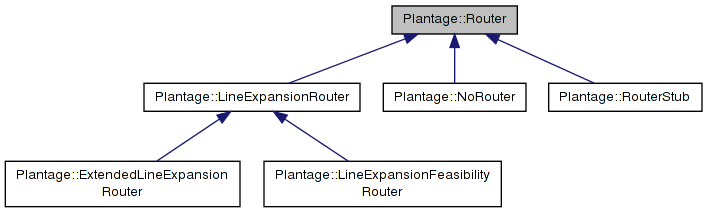
\includegraphics[scale=.6]{FIG/class_diagram_router.png}  	
	\caption{inheritance diagram for the router}	
	\label{fig:class_diagram_router}
\end{figure}

The results above show that the layouts created by Plantage are at least feasible. Additionally, they also consider several constraints for analog circuits. The results are certainly not perfect yet, but this wasn't the aim of this thesis. The real main point was to implement the routing and make it easy to replace the algorithm later, as it is not certain which solution will be the best for the hierarchical placer. This can now easily be done; it is only necessary to inherit from the class Router.

\begin{samepage}
Finally, I was able to reach all the targets claimed in the introduction:
\begin{itemize}
\item a line expansion router, which creates, in most cases \footnote{In the cases where the layout is not design rule clean it is usually easy to fix the problem manually. For instance, in special cases the minimum notch rule may be harmed, but then the gap can just be filled up.}, design rule clean routes \footnote{For the capacitor the ICFBInterface does not provide enough information on the additional guard ring, therefore it cannot be considered} and considers symmetries
\item based on the previous router an extended version, which tries to reduce the parasitics
\item a software design, where the routing algorithm can be exchanged easily
\end{itemize}
\end{samepage}

\begin{figure}
	\centering	
	\subfloat[basic line expansion router]{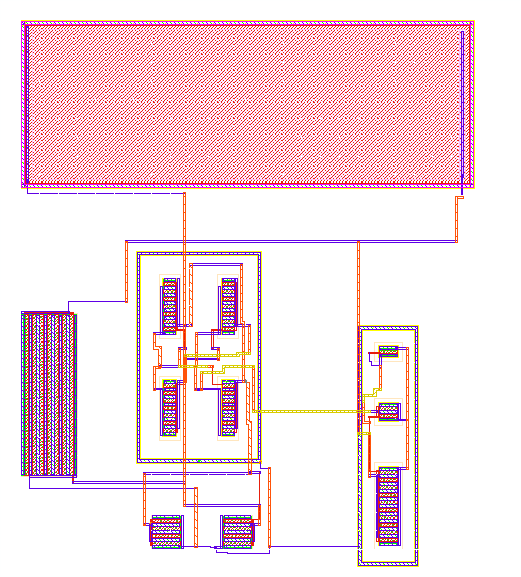
\includegraphics[scale=0.6]{FIG/miller_amplifier_routed_basic_line_expansion.png}}	
	\subfloat[extended line expansion router]{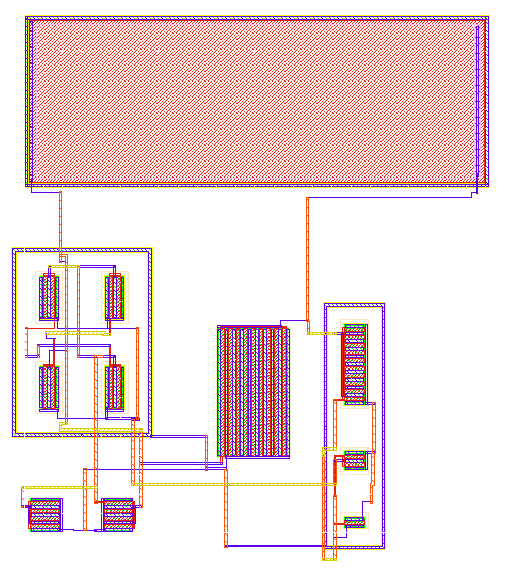
\includegraphics[scale=0.6]{FIG/miller_amplifier_routed_extended_line_expansion.png}}	
	\caption{two similar placements routed}	
	\label{fig:miller_amplifier_routed_line_expansion_router}
\end{figure}

\begin{figure}	
	\centering	
	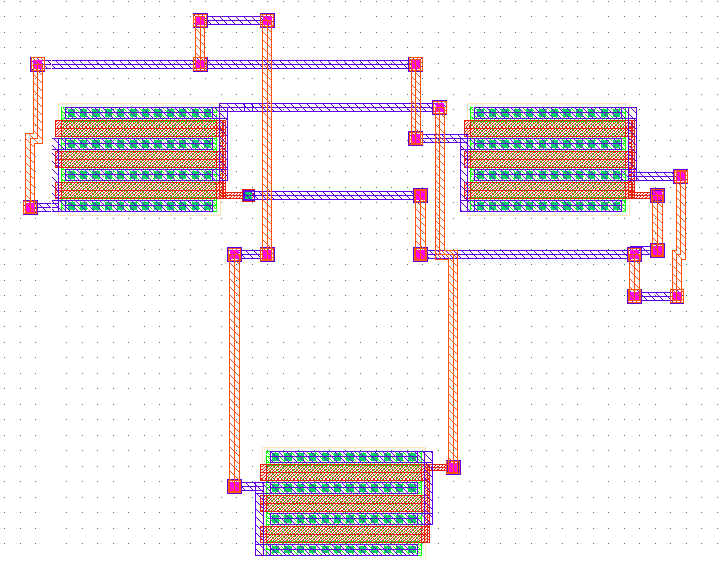
\includegraphics[scale=.6]{FIG/symmetry_routed.png}  	
	\caption{routed layout of a symmetry}	
	\label{fig:symmetry_routed}
\end{figure}

\begin{figure}	
	\centering	
	\subfloat[basic line expansion router]{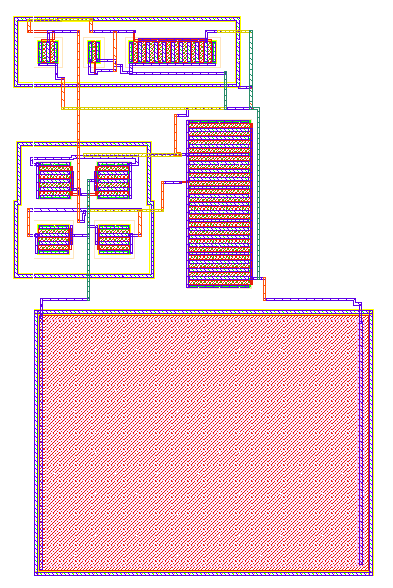
\includegraphics[scale=0.75]{FIG/miller_amplifier_routed_smaller_basic_line_expansion.png}}	
	\subfloat[extended line expansion router]{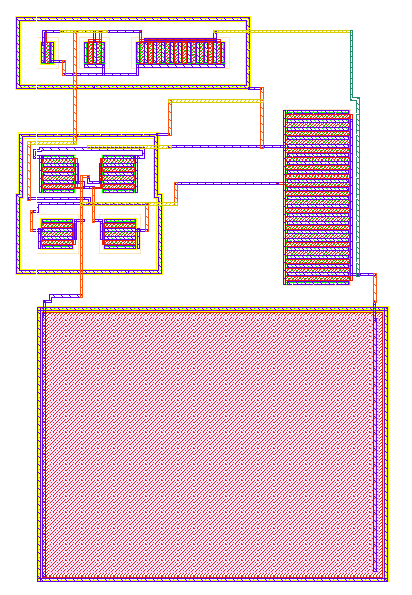
\includegraphics[scale=0.75]{FIG/miller_amplifier_routed_smaller_extended_line_expansion.png}}
	\caption{two similar placements without a common centroid routed}	
	\label{fig:miller_amplifier_smaller_routed_line_expansion_router}
\end{figure}